\chapter{Calcolo della Relatedness}

La seconda parte del progetto riguarda l'analisi di due metodi critici (\code{readDump()} e \code{rel(int a, int b)}) che servono a 
calcolare, dati gli identificativi di due entità semantiche, il loro valore di correlazione (relatedness). 

Per fare ciò si ha a disposizione un dump dove sono salvati tutti i valori di correlazione (sopra una certa soglia minima) per ogni coppia di entità. 

Il metodo \code{readDump()} serve a caricare in memoria i valori del dump 
sottoforma di \lq\lq matrice\rq\rq\ mentre il metodo \code{rel(int a, int b)} serve a fare una ricerca nella struttura dati per poi ritornare il valore di 
correlazione fra le entità con identificativi \code{a} e \code{b}.

Questa scelta implementativa, attualmente adottata, è sicuramente molto efficiente in termini di prestazioni ma sicuramente molto onerosa in termini di memoria; 
pertanto il fine dell'analisi sarebbe quello di studiare/testare implementazioni alternative per ottimizzare le prestazioni e/o diminuire lo spreco di memoria.  

%%%%%%%%%%%%%%%%%%%%%%%%%%%%%%%%%%%%%%%%%%%%%%%%%%%%%%%%%%%%%%%%%%%%%%%%%%%%%%%%%%%%%%%%%%%%%%%%%%%%%%%%%%%%%%%%%%%%%%%%
\section{Implementazione Iniziale}

%%%%%%%%%%%%%%%%%%%%%%%%%%%%%%%%%%%%%%%%%%%%%%%%%%%%%%%%%%%%%%%%%%%%%%%%%%%%%%%%%%%%%%%%%%%%%%%%%%%%%%%%%%%%%%%%%%%%%%%%
\subsection{Il Dump}
\begin{lstlisting}[style=TeXStyle, caption=Estratto del dump]
53676192
4922289
0.01
2
1.0
53676158 7 null
53676164 5 NnAwQT/ZvTVJ05MeSfcdI0rMrg1LBmUH
53676016 13 RDsFRUkyASRLFf3T
53675811 16 null
...
\end{lstlisting}

Leggendo le prime righe di un dump si nota che le prime cinque righe sono valori di inizializzazione mentre dalla sesta righa in poi troviamo le righe della matrice.
Il primo numero intero, denominato \textit{max$\_$id}, indica il limite massimo che gli id delle entità possono assumere; 
dato che gli id delle entità non sono necessariamente sequenziali 
(fra due di essi potrei avere dei \lq\lq buchi\rq\rq, degli intervalli in cui gli identificativi non sono associati ad alcuna entità) 
esiste una funzione \textit{map} che mappa (\lq\lq compatta\rq\rq) gli id delle entità su altri id univoci e sequenziali. 

Il secondo intero, denominato \textit{nodesSize} è il valore massimo che la funzione \textit{map} può assumere (limita il codominio della funzione).

\begin{equation}\begin{split}
    map():\ \mathbb{N} & \rightarrow \mathbb{N}\\
            [0,max\_id] & \rightarrow [0, nodeSize], max\_id \geq nodeSize\\
\end{split}\end{equation}

Continuando a leggere il dump troviamo la relatedness minima considerata \textit{minRel} (sotto la quale i valori di correlazione non vengono salvati) 
e altri valori di configurazione quali \textit{minIntersection} e \textit{threshold} che tuttavia non ci interessano particolarmente.

La funzione map in un certo senso mappa \lq\lq al contrario\rq\rq\ gli id; infatti l'id massimo verrà mappato su 0, il penultimo id verrà mappato su 1 e così via.
Nel caso del dump in questione abbiamo:

\begin{lstlisting}[style=TeXStyle, caption=Esempio di funzione map e postingList]
MaxId = 53676192
NodeSize = 4922289

   ID		        MAP(ID)    POSTINGLIST
...
53676158    ->      7           null
53676159    ->      6           FW/I...
53676164    ->      5           NnAw...
53676174    ->      4           null
53676176    ->      3           null
53676177    ->      2           null
53676180    ->      1           null
53676190    ->      0           null
\end{lstlisting}

Gli id presenti nel dump non sono ordinati ma le \textit{postingList} ad essi associate lo sono.

Dalla sesta riga del dump in poi inizia la definizione della matrice, ogni riga è composta da tre valori separati da uno spazio. 
Ad esempio se consideriamo la riga:
\begin{lstlisting}[style=TeXStyle, caption=Riga del dump]
53676164 5 NnAwQT/ZvTVJ05MeSfcdI0rMrg1LBmUH
\end{lstlisting}

Il primo valore $a = 53676164$ è l'id di un entità, il secondo valore $b = 5 = map(a)$ è il risultato della funzione map, 
infine il terzo valore $c = NnAwQT/ZvTVJ05MeSfcdI0rMrg1LBmUH$ è una stringa di dimensione variabile oppure \textit{null};
quest'ultima stringa, denominata \textit{postingList}, è la codifica in \textit{Base64} di un array di byte che rappresenta un dizionario chiave valore. 

\begin{center}
    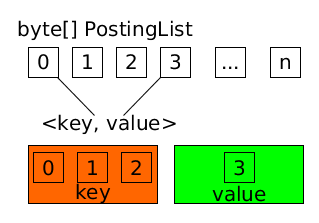
\includegraphics[scale=0.55]{Sources/Img/c02_01.png}
    \captionof{figure}{Encoding del dizionario nella postingList}
\end{center}

In pratica una tupla $<chiave,\ valore>$ è codificata sull'array da una sequenza di quattro byte; quindi partizionando l'array in gruppi da 4 byte 
ottengo, per ogni gruppo, la chiave (è un id \lq\lq mappato\rq\rq ) codificata sui primi tre byte ed il valore (la relatedness) definito sul quarto byte (il byte più a destra).

Questa codifica, pertanto, permette di gestire set di entità con id \lq\lq mappato\rq\rq\ massimo $2^{3 \cdot 8} \simeq 1,7 \cdot 10^7$ ed una scala di valori 
di correlazione appartenenti all'intervallo $[0,\ 255]$.

Bisogna precisare che l'array di byte, denominato \textit{postingList}, è ordinato per valore crescente delle chiavi e, dato che rel(a, b) = rel(b, a),
si è deciso di salvare una sola volta il valore di correlazione imponendo la relazione: $a > b$.

%%%%%%%%%%%%%%%%%%%%%%%%%%%%%%%%%%%%%%%%%%%%%%%%%%%%%%%%%%%%%%%%%%%%%%%%%%%%%%%%%%%%%%%%%%%%%%%%%%%%%%%%%%%%%%%%%%%%%%%%
\subsubsection{Esempio}
Nell'ipotesi in cui abbia una riga nel dump costituita dalla tupla $(a,\ b,\ c)$ e volessi trovare $relatedness(a, d)$ con $map(a) > map(d)$. 

Devo cercare nella \textit{postingList c}, un gruppo di quattro byte in cui i primi tre byte corrispondano a \textit{map(d)} ed il quarto byte sarà il valore di correlazione voluto. 

Ovviamente è possibile che \textit{c} sia \textit{null} (l'entità con id \textit{a} non ha nessuna correlazione con entità i cui id \lq\lq mappati\rq\rq\ siano inferiori a \textit{b}) oppure 
che nella posting non sia presente nessuna chiave corrispondente a \textit{map(d)}, in questi casi $relatedness(a,d) = 0$. 

%%%%%%%%%%%%%%%%%%%%%%%%%%%%%%%%%%%%%%%%%%%%%%%%%%%%%%%%%%%%%%%%%%%%%%%%%%%%%%%%%%%%%%%%%%%%%%%%%%%%%%%%%%%%%%%%%%%%%%%%
\subsection{Il Codice Nativo}

\begin{lstlisting}[style=JavaStyle, caption=Implentazione nativa]
// STRUTTURA DATI
public class RelatednessMatrix {
    public int[] map;
    public byte[][] matrix;
    public float configuredMinRel;
    public int configuredMinIntersection;
    public float threshold;
    public static int EL_SIZE = 4;
}

// CODICE UTILIZZO
public float rel(int a, int b){
    if(a==b) return 1f;

    int nodeA = data.map[a];
    int nodeB = data.map[b];
    if (nodeA < 0 || nodeB < 0) return 0f;

    int key = a>b ? nodeB : nodeA;
    byte[] array = a>b ? data.matrix[nodeA] : data.matrix[nodeB];

    if (array == null) return 0f;

    int start = 0;
    int end = array.length - RelatednessMatrix.EL_SIZE;
    int pos = -1;
    while(pos == -1 && start <= end)
    {
        int idx = ((start+end)/RelatednessMatrix.EL_SIZE)/2;
        int idx_value = ((array[idx*RelatednessMatrix.EL_SIZE] & 0xFF) << 16)
                    + ((array[idx*RelatednessMatrix.EL_SIZE+1] & 0xFF) << 8)
                    + ( array[idx*RelatednessMatrix.EL_SIZE+2] & 0xFF);

        if(idx_value == key) pos = idx;
        else{
            if(key > idx_value)
                start = (idx + 1) * RelatednessMatrix.EL_SIZE;
            else
                end = (idx - 1) * RelatednessMatrix.EL_SIZE;
        }
    }

    if(pos == -1) return 0f;
    else
    {
        byte by = array[pos * RelatednessMatrix.EL_SIZE + 3];
        int byint = by + 128;
        float byteRel = byint / 255f;
        return data.configuredMinRel + byteRel * (1 - data.configuredMinRel);
    }
}

// CODICE LETTURA
public String END_OF_FILE = "" + '\0';

public RelatednessMatrix readDump() throws Exception {
    URL url = getClass().getResource("dump.txt");
    File file = new File(url.getPath());
    BufferedReader fbr = new BufferedReader(new FileReader(file));
    String line = new String();

    try {   
        int max_id = Integer.parseInt(fbr.readLine().trim()); // Trims all leading and trailing whitespace from this string         
        int nodesSize = Integer.parseInt(fbr.readLine().trim());
        float minRel = Float.parseFloat(fbr.readLine().trim());
        int minIntersection = Integer.parseInt(fbr.readLine().trim());
        float threshold = Float.parseFloat(fbr.readLine().trim());         

        RelatednessMatrix data = new RelatednessMatrix();
        data.map = new int[max_id + 1];
        data.matrix = new byte[nodesSize][];
        data.configuredMinRel = minRel;
        data.configuredMinIntersection = minIntersection;
        data.threshold = threshold;

        int idx = 0;

        while ((line = fbr.readLine()) != null) {
            if (line.trim().equals(END_OF_FILE.trim())) {
                break;
            }
            System.out.println(line);
            String[] splittedLine = line.split("\\s+"); // split(" ")
            if (splittedLine.length != 3) {
                throw new Exception("Wrong format relatedness file for the line: " + line);
            }

            int wid = Integer.parseInt(splittedLine[0]);
            int node = Integer.parseInt(splittedLine[1]);
            data.map[wid] = node;

            if (splittedLine[2].equals("null")) {
                data.matrix[node] = null;
            } else {
                byte[] a = Base64.getDecoder().decode(splittedLine[2].toString()); 
                data.matrix[node] = Base64.getDecoder().decode(splittedLine[2].toString());
            }
            idx++;
        }
        
        if (idx != nodesSize) {
            throw new Exception("Wrong format relatedness file the number of line do not match with size of matrix");
        }
        
        return data;
    } catch (Exception e) {
        System.out.println(e.getMessage());
        return null;
    }
}
\end{lstlisting}

Il metodo \code{readDump()} legge riga per riga il dump e restituisce un'istanza di RelatednessMatrix valorizzata. 
La funzione map viene salvata in un array di interi (\code{data.map}) mentre la matrice con le correlazioni viene salvata in un 
array bidimensionale di byte (\code{data.matrix}).

Il metodo \code{rel(int a, int b)} invece calcola la funzione \code{map} sugli id \code{a} e \code{b} dopodichè fa una binary search sulla postingList 
ottenuta da matrix[map(a)] (assumendo $map(a) > map(b)$). Infine se la ricerca binaria ha successo il valore di relatedness ottenuto va riscalato su una scala di valori 
$[0, 255]$, convertito in float e riscalato nuovamente in base al valore di relatedness minima considerata (per escludere i valori al di sotto della relatedness minima,
che non verranno mai usati).  

\begin{lstlisting}[style=JavaStyle, caption=Conversione della relatedness da byte a float]
byte by = array[pos * RelatednessMatrix.EL_SIZE + 3]; //considero il quarto byte 
int byint = by + 128;   //scalo di 128 valori per ottenere una relatedness in [0, 255]

//cast in float, escludendo i valori sotto la relatedness minima (configuredMinRel)
float byteRel = byint / 255f; 
return data.configuredMinRel + byteRel * (1 - data.configuredMinRel);
\end{lstlisting}

%%%%%%%%%%%%%%%%%%%%%%%%%%%%%%%%%%%%%%%%%%%%%%%%%%%%%%%%%%%%%%%%%%%%%%%%%%%%%%%%%%%%%%%%%%%%%%%%%%%%%%%%%%%%%%%%%%%%%%%%
\subsection{Osservazioni}
Considerato che il metodo \code{readDump()} viene chiamato una sola volta per allocare in memoria la struttura dati nel server, 
non ci sono particolari vincoli temporali per la sua esecuzione; per quanto riguarda il calcolo della relatedness invece 
l'algoritmo dev'essere il più performane possibile.

Il codice nativo per il calcolo della relatedness costa $O(lg_2(n))$ (con $n=nodeSize$) per la ricerca binaria e O(1) per quanto riguarda le 
istruzioni precedenti e successive a quest'ultima.

Tolto un piccolo refact del codice che portebbe ad evitare tre moltiplicazione per ciclo nella binary search (non è necessario dividere e poi moltiplicare per 
RelatednessMatrix.EL$\_$SIZE), non sembra si possono migliorare di molto le prestazioni dell'algoritmo senza cambiare struttura dati.

Una via percorribile per non \lq\lq pagare\rq\rq\ $O(lg_2(n))$ per la binary search potrebbe essere quella di allocare direttamente in memoria la matrice 
completa (in questo caso avrei un algoritmo di tempo costante O(1)). Questa soluzione però andrebbe a peggiorare drasticamente lo spreco di memoria.
Infatti nell'implementazione attuale la matrice ha dimensione massima $nodeSize \otimes nodeSize$ ma le righe hanno dimensione variabile e 
non occupano quindi sempre $(nodeSize -1) \cdot 4\ Byte$.

%%%%%%%%%%%%%%%%%%%%%%%%%%%%%%%%%%%%%%%%%%%%%%%%%%%%%%%%%%%%%%%%%%%%%%%%%%%%%%%%%%%%%%%%%%%%%%%%%%%%%%%%%%%%%%%%%%%%%%%%
\subsubsection{Stima della Memoria Allocata}
Se consideriamo le prime righe del dump in questione possiamo stimare che mediamente il $57\%$ degli id hanno postingList vuota (null) ed il restante $43\%$ ha un numero 
medio di relatedness per id pari allo $0,000101\%$ di nodeSize.

L'implementazione attuale alloca in memoria per l'array di interi map circa:
\begin{center}
\begin{equation}\begin{split} 
    nodeSize \cdot 4\ Byte & = 4^2 \cdot 10^6 Byte = 16 MB \\
\end{split}\end{equation}
(arrotondando e senza tenere conto di fattori secondari come i 32 byte occupati da overhead e puntatore).
\end{center}
Per la matrice invece possiamo assumere che, su una macchina a 64 bit, avrò il $57\%$ di righe a null ($0.57 \cdot 4\cdot 10^6 \cdot 8\ Byte = 18\ MB$) ed il 
restante $43\%$ di righe con mediamente 404 valori di relatedness codificati su 4 Byte ($0.43 \cdot 4 \cdot 10^6 \cdot 404 \cdot 4\ Byte = 2.8\ GB$). 

Quindi in totale potremmo stimare che solo questo dump occupa quasi 3 GB (notare che esiste un dump per ogni lingua supportata da Dandelion e che questo è uno 
dei dump più piccoli).

%%%%%%%%%%%%%%%%%%%%%%%%%%%%%%%%%%%%%%%%%%%%%%%%%%%%%%%%%%%%%%%%%%%%%%%%%%%%%%%%%%%%%%%%%%%%%%%%%%%%%%%%%%%%%%%%%%%%%%%%
\subsubsection{Stima della Matrice Completa}
Se allocassimo in memoria una matrice di Byte completa, di dimensioni $nodeSize \otimes nodeSize$, essa occuperebbe $(4 \cdot 10^6)^2 = 1.6 \cdot 10^{13}\ Byte = 16\ TB$.
Pur considerando che esistono strutture dati particolarmente ottimizzate per gestire array di grandi dimensioni con pochi valori al loro interno (teniamo presente che
più della metà dei valori nella matrice non saranno valorizzati), come SparseArray e SuperArrayList, bisogna tener presente che spesso tali strutture dati 
si basano su liste; in questo caso però difficilmente si otterrebbero prestazioni migliori di quelle dell'implementazione attuale dato che il tempo di lookup 
sarebbe sempre $O(lg_2(noseSize))$. 

In conclusione, a meno di uno spreco di memoria ulteriore, difficilmente otterremo buoni risultati mantenendo come struttura dati di riferimento la matrice. 

%%%%%%%%%%%%%%%%%%%%%%%%%%%%%%%%%%%%%%%%%%%%%%%%%%%%%%%%%%%%%%%%%%%%%%%%%%%%%%%%%%%%%%%%%%%%%%%%%%%%%%%%%%%%%%%%%%%%%%%%
\subsubsection{Stima del problema inverso}
Una via praticabile potrebbe essere quella di vedere il problema al contrario, considerando che esistono solo 256 valori possibili di relatedness, 
per minimizzare lo spreco di memoria potrei pensare di allocare 256 array in cui storicizzo tutte le coppie di id che hanno la stessa relatedness. 
In questo modo eliminerei la ridondanza costituita da valori uguali di relatedness salvati nel dump migliaia di volte.

Ci si accorge subito che anche questa via non è praticabile dato che per risparmiare 1 Byte devo storicizzare 8 Byte per le coppie di id di tipo intero. 
Andrei ad occupare $0.43 \cdot 4 \cdot 10^6 \cdot 404 \cdot 2 \cdot 4 = 5.6 GB$, il doppio rispetto all'implementazione nativa, senza contare che 
le performance peggiorerebbero.

%%%%%%%%%%%%%%%%%%%%%%%%%%%%%%%%%%%%%%%%%%%%%%%%%%%%%%%%%%%%%%%%%%%%%%%%%%%%%%%%%%%%%%%%%%%%%%%%%%%%%%%%%%%%%%%%%%%%%%%%
\subsubsection{Stima implementazione di un grafo}
Si potrebbe pensare di implementare un grafo orientato, salvando per ogni nodo l'id e la lista di archi uscenti e su ogni arco la relatedness fra nodo di partenza 
e nodo di arrivo. Dovrei quindi usare una struttura dati del tipo:
 
\begin{lstlisting}[style=JavaStyle]
    public class Node{
        public int Id;
        public List<Arrow> Arrows;  
    }

    public class Arrow{
        public Node Node;
        public byte Relatedness;
    }
\end{lstlisting}

Tuttavia in questo modo sprecherei memoria perchè il puntatore al nodo successivo (ipotizzando di lavorare su una macchina a 64 bit) peserebbe più dell'identificativo 
del nodo stesso. Al che potrei sostituire il puntatore con un intero ma anche in questo caso avrei il dizionario $< Id,\ Relatedness >$ che pesa 5 Byte mentre nella 
postingList pesa 4 Byte perchè chiave e valore sono accorpati. Infine se seguissi la stessa politica di codifica del dizionario della postingList 
di fatto sarei tornato all'implementazione iniziale senza trarre alcun giovamento, se non lo svantaggio agguintivo di non poter accedere in O(1) ad un nodo arbitrario. 

%%%%%%%%%%%%%%%%%%%%%%%%%%%%%%%%%%%%%%%%%%%%%%%%%%%%%%%%%%%%%%%%%%%%%%%%%%%%%%%%%%%%%%%%%%%%%%%%%%%%%%%%%%%%%%%%%%%%%%%%
\section{Implementazione con Hash Map}
Sembra che l'unica via praticabile per mantenere tutti i dati in memoria, diminuendo la memoria occupata e massimizzando le prestazioni sia una funzione di Hash Map, 
che mappi gli id concatenati sul valore della relatedness; se la funzione fosse ben ottimizzata otterrei in O(1) la relatedness (guadagno prestazionale)
e potenzialmente potrebbe occupare meno memoria della matrice iniziale.

Purtroppo è molto difficile stimare a priori lo spazio occupato da un Hash Map, 
il modo più rapido è confrontare con dei benchmark l'implementazione nativa contro quella basata su Hash Map.

\subsection{Codice}
\begin{lstlisting}[style=JavaStyle, caption=Implentazione con HashMap]
public float Relatedness(int a, int b) throws Exception {
    if (a == b) {
        return 1f;
    }

    int nodeA = data.map[a];
    int nodeB = data.map[b];

    if (nodeA < 0 || nodeB < 0) {
        return 0f;
    }

    String key = (nodeA > nodeB) ? (nodeA + "." + nodeB) : (nodeB + "." + nodeA);
    try {
        byte value = (byte) data.hm.get(key);

        if (value == 0) {
            return 0f;
        } else {
            int byint = value + 128;
            float byteRel = byint / 255f;
            return data.configuredMinRel + byteRel * (1 - data.configuredMinRel);
        }
    } catch (Exception e) {
        return 0f;
    }
}

public RelatednessHashMap ReadDump(String dump) throws Exception {
    URL url = getClass().getResource(dump);
    File file = new File(url.getPath());
    BufferedReader fbr = new BufferedReader(new FileReader(file));
    String line = new String();

    try {
        RelatednessHashMap data = new RelatednessHashMap();
        int max_id = Integer.parseInt(fbr.readLine().trim());
        int nodesSize = Integer.parseInt(fbr.readLine().trim());
        data.configuredMinRel = Float.parseFloat(fbr.readLine().trim());
        data.configuredMinIntersection = Integer.parseInt(fbr.readLine().trim());
        data.threshold = Float.parseFloat(fbr.readLine().trim());

        data.map = new int[max_id + 1];
        data.hm = new HashMap();

        String END_OF_FILE = "" + '\0';

        while ((line = fbr.readLine()) != null) {
            if (line.trim().equals(END_OF_FILE.trim())) {
                break;
            }

            String[] splittedLine = line.split("\\s+");
            if (splittedLine.length != 3) {
                throw new Exception("Wrong format relatedness file for the line: " + line);
            }

            int wid = Integer.parseInt(splittedLine[0]);
            int node = Integer.parseInt(splittedLine[1]);
            data.map[wid] = node;

            if (!splittedLine[2].equals("null")) {
                byte[] postingList = Base64.getDecoder().decode(splittedLine[2].toString());

                int idx_value = ((postingList[0] & 0xFF) << 16)
                            + ((postingList[1] & 0xFF) << 8)
                            + ((postingList[2] & 0xFF) << 0);

                String key = idx_value + "." + node;
                data.hm.put(key, postingList[3]);
            }
        }

        return data;
    } catch (Exception e) {
        System.out.println(e.getMessage());
        return null;
    }
}
\end{lstlisting}

[\textbf{TODO} implementazione alternativa fastutils e metrics di Prometheus e Grafana]